\section{Vector Fields}
Vector field is a function whose domain is a set of points in $\R^n$ and whose range is a set of vectors in $V_n$. In other words, a vector field assigns to each point in $\R^n$ a vector.

\begin{definition}[Vector fields]
Let $S$ be a subset of $\R^n$. A vector field in $\R^n$ is a function $\vv F:\; S \to \R^n$.
\end{definition}

Vector fields are often used in physics. Some examples include gravitational field and electric field.

\begin{example}[Gravitational fields and electric fields]
\hfill \\
Gravitational field:
$$
\vv{F}(\vv x) = - \frac{mMG}{\norm{\vv x}^3}\vv x
$$
Electric field:
$$
\vv{E}(\vv x) = \frac{\varepsilon Q}{\norm{\vv x}^3}\vv x
$$
\end{example}

\section{Graident, Divergence, and Curl}

\subsection{Definitions}

\begin{definition}[Gradient]
Let $f(x,y,z)$ be differentiable at each point in certain region of space. Then the gradient of $f(x,y,z)$, written $\nabla f$, is defined by
$$
\nabla f = \left( \partialderiv{}{x}\vv i + \partialderiv{}{y}\vv j + \partialderiv{}{z}\vv k \right) f = \left( \partialderiv{f}{x}, \partialderiv{f}{y}, \partialderiv{f}{z} \right)
$$
\end{definition}

\begin{definition}[Divergence]
Let $\vv F (x,y,z) = (P(x,y,z), Q(x,y,z), R(x,y,z))$ be defined and differentiable at each point in certain region of space (i.e. $\vv F$ defines a differentiable vector field). Then the divergence of $\vv F$, written $\nabla \cdot \vv F$, or $\mathrm{div} \vv F$ is defined by
$$
\nabla \cdot \vv F = \left( \partialderiv{}{x}\vv i + \partialderiv{}{y}\vv j + \partialderiv{}{z}\vv k \right) \cdot (P,Q,R) = \partialderiv{P}{x} + \partialderiv{Q}{y} + \partialderiv{R}{z}
$$
The divergence of a vector field is a scalar field.
\end{definition}

\begin{definition}[Curl]
If $\vv F (x,y,z) = (P(x,y,z), Q(x,y,z), R(x,y,z))$ is a differentiable vector space. Then the curl of $\vv F$, written $\nabla \times \vv F$, or $\mathrm{curl} \vv F$ is defined by
$$
\nabla \times \vv F = \left( \partialderiv{}{x}\vv i + \partialderiv{}{y}\vv j + \partialderiv{}{z}\vv k \right) \times (P,Q,R)
$$
The curl can be represented in determinant notation as
$$
\nabla \times \vv F = \begin{vmatrix}
\vv i & \vv j & \vv k \\
\partialderiv{}{x} & \partialderiv{}{y} & \partialderiv{}{z} \\
P & Q & R
\end{vmatrix} = \left(\partialderiv{R}{y}-\partialderiv{Q}{z},\, \partialderiv{P}{z}-\partialderiv{R}{z},\, \partialderiv{Q}{x}-\partialderiv{P}{y} \right)
$$
The curl of a vector field defines a vector field.
\end{definition}

\subsection{Geometric Interpretation}
Geometrically, given a point, the divergence tells us whether a particle at that point tends to diverge or converge, and by how much. More technically, the divergence represents the volume density of the outward flux of a vector field from an infinitesimal volume around a given point. When $\Div \vv F = 0$, then $\vv F$ is said to be \textit{incompressible}.

\begin{figure}[h]
    \centering
    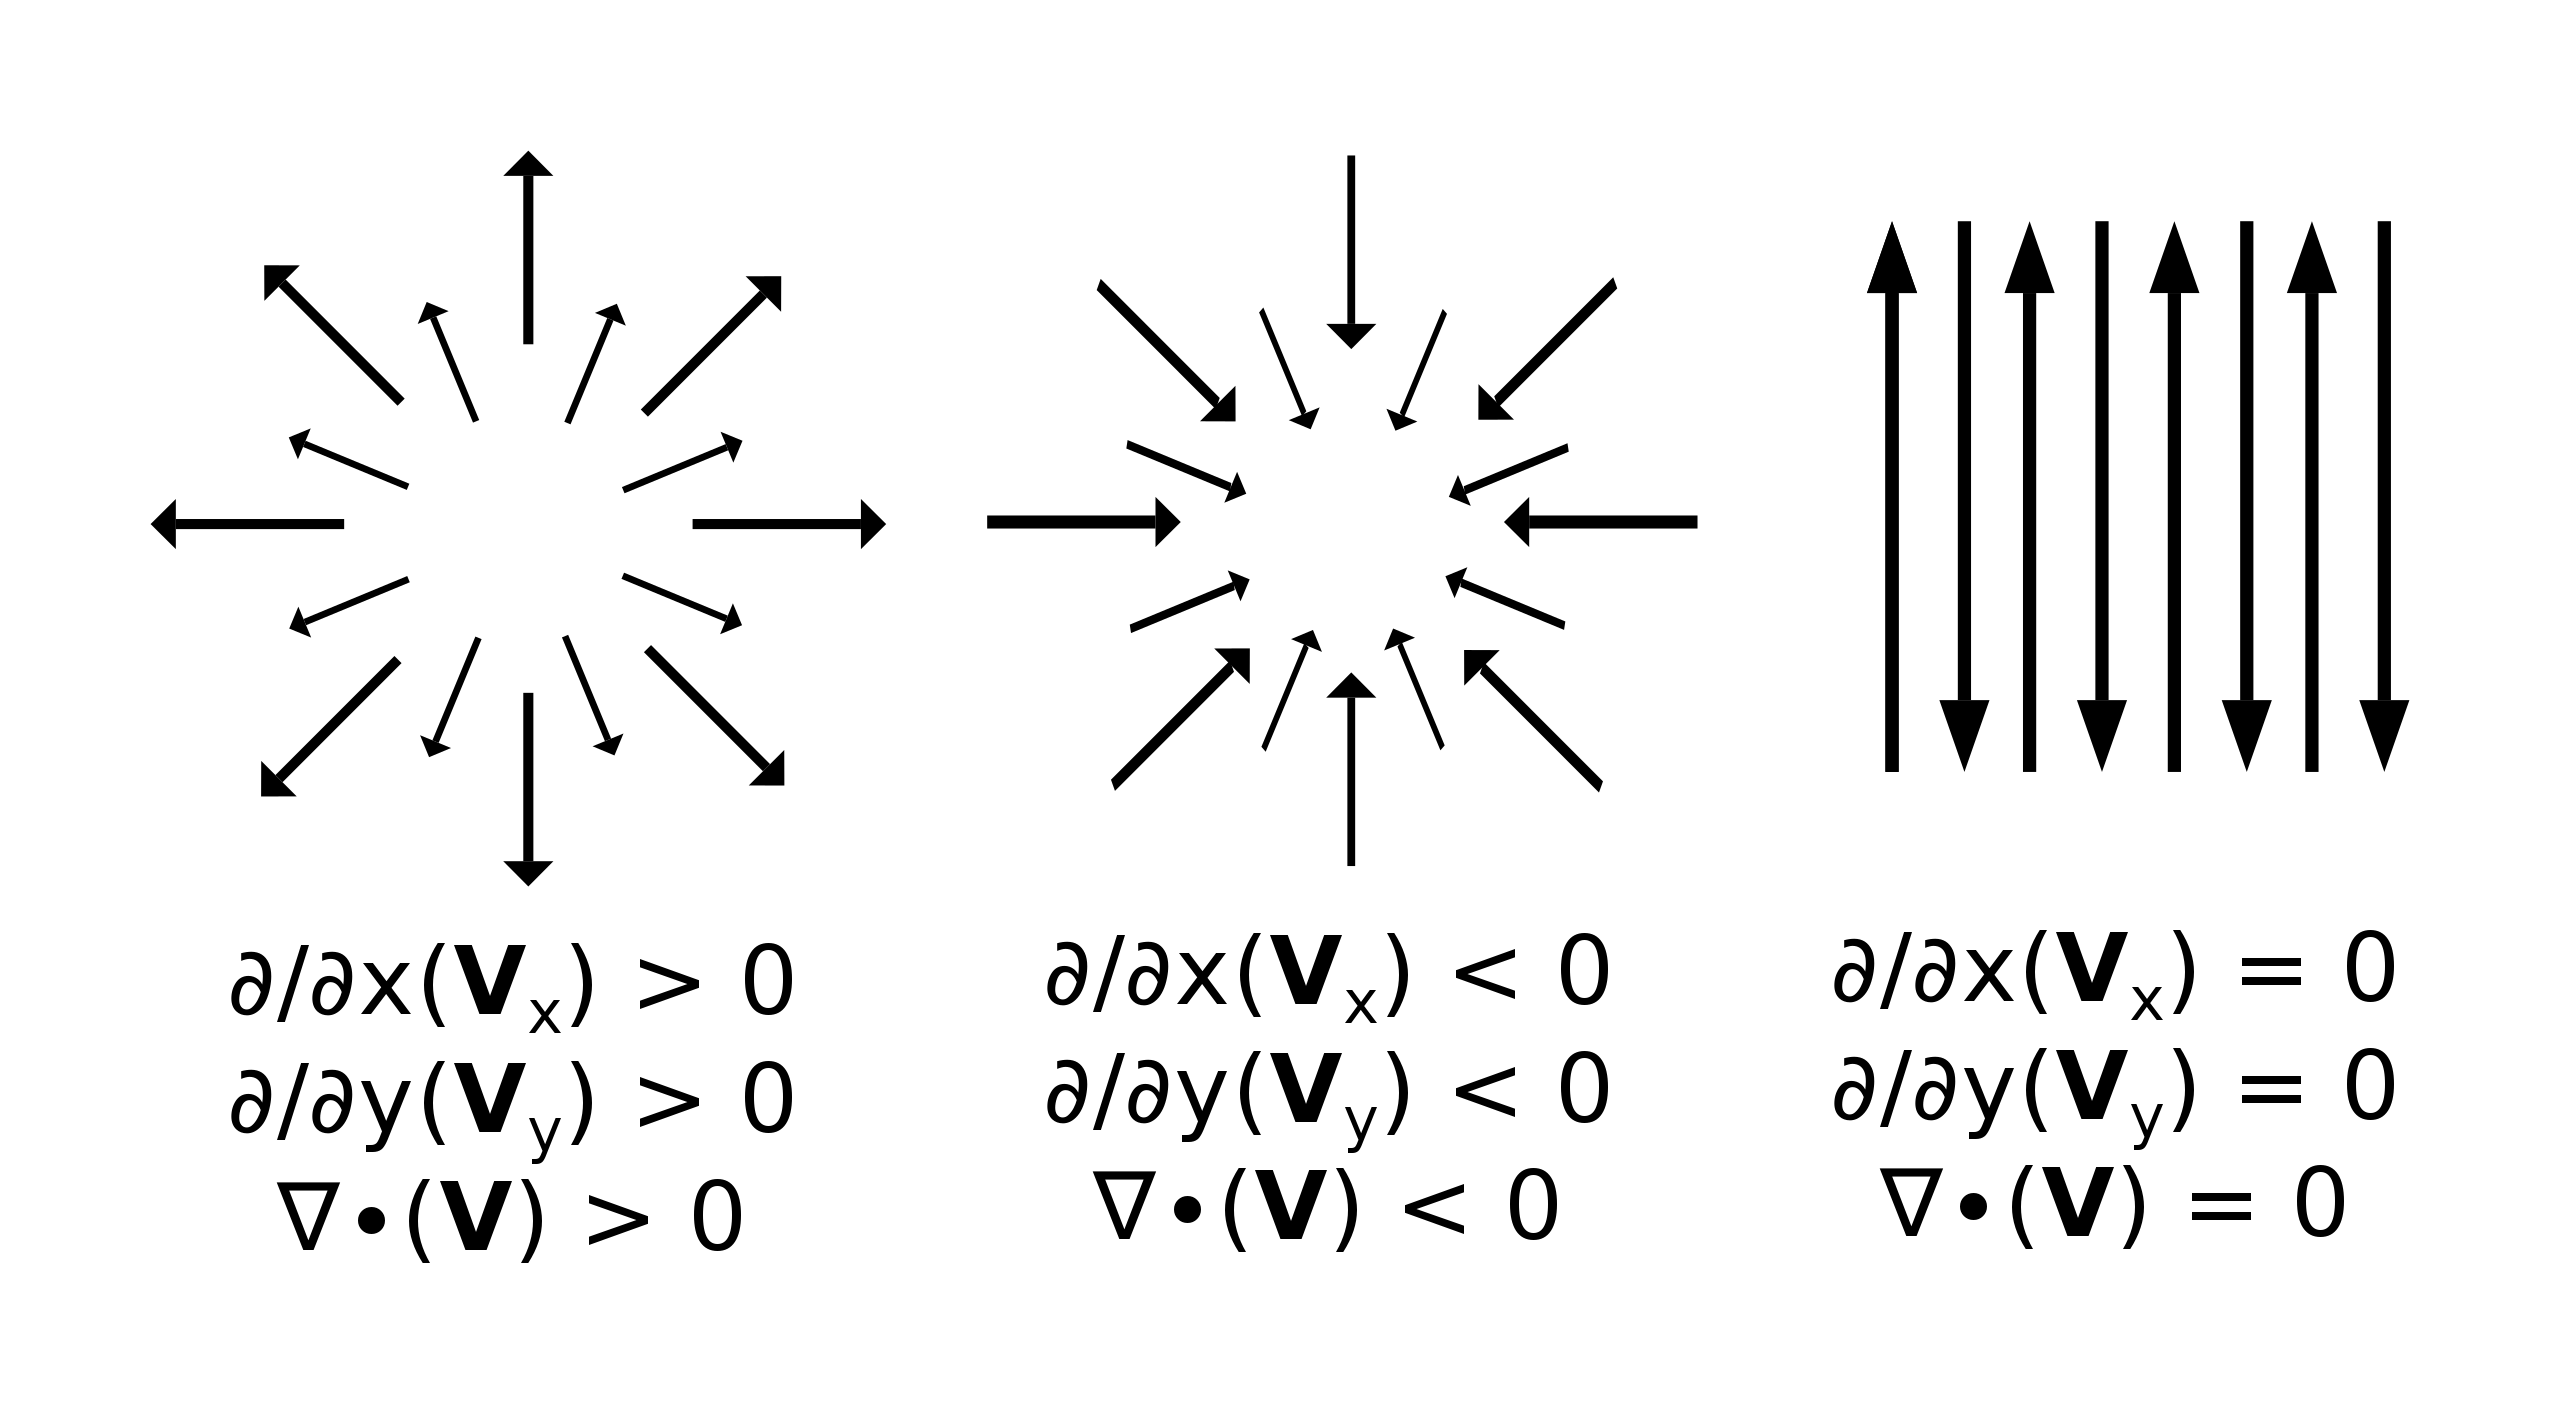
\includegraphics[width=0.5\linewidth]{figures/divergence.png}
    \caption{A positive divergence indicates that particles tend to diverge away from that point; a negative divergence indicates that particles tend to converge at that point; a zero divergence means that there is no net density change at that point.}
    \label{fig:divergence}
\end{figure}

Curl is geometrically associated with rotation of particles in a vector field. Curl tells us the direction of rotation at a given point. To determine the direction of the curl, we use the right-hand rule just like when we are determining the angular momentum of a rotating object. Imagine curling your right hand around the direction of rotation and stick up your thumb, your thumb should point in the direction of the curl.

\begin{figure}[h]
    \centering
    \raisebox{-0.5\height}{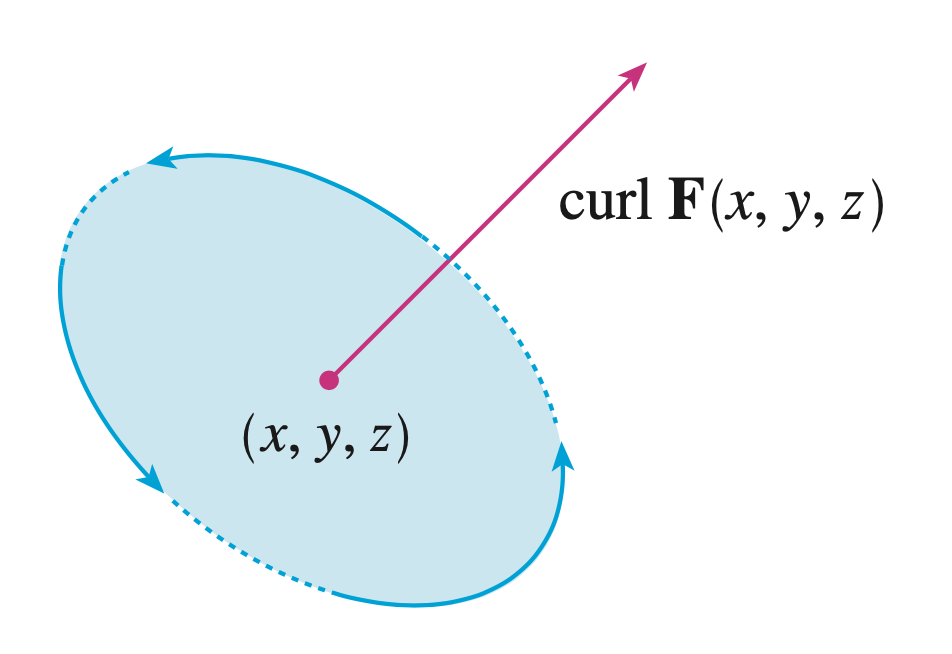
\includegraphics[width=0.25\linewidth]{figures/curl-simple.png}}
    \qquad
    \raisebox{-0.5\height}{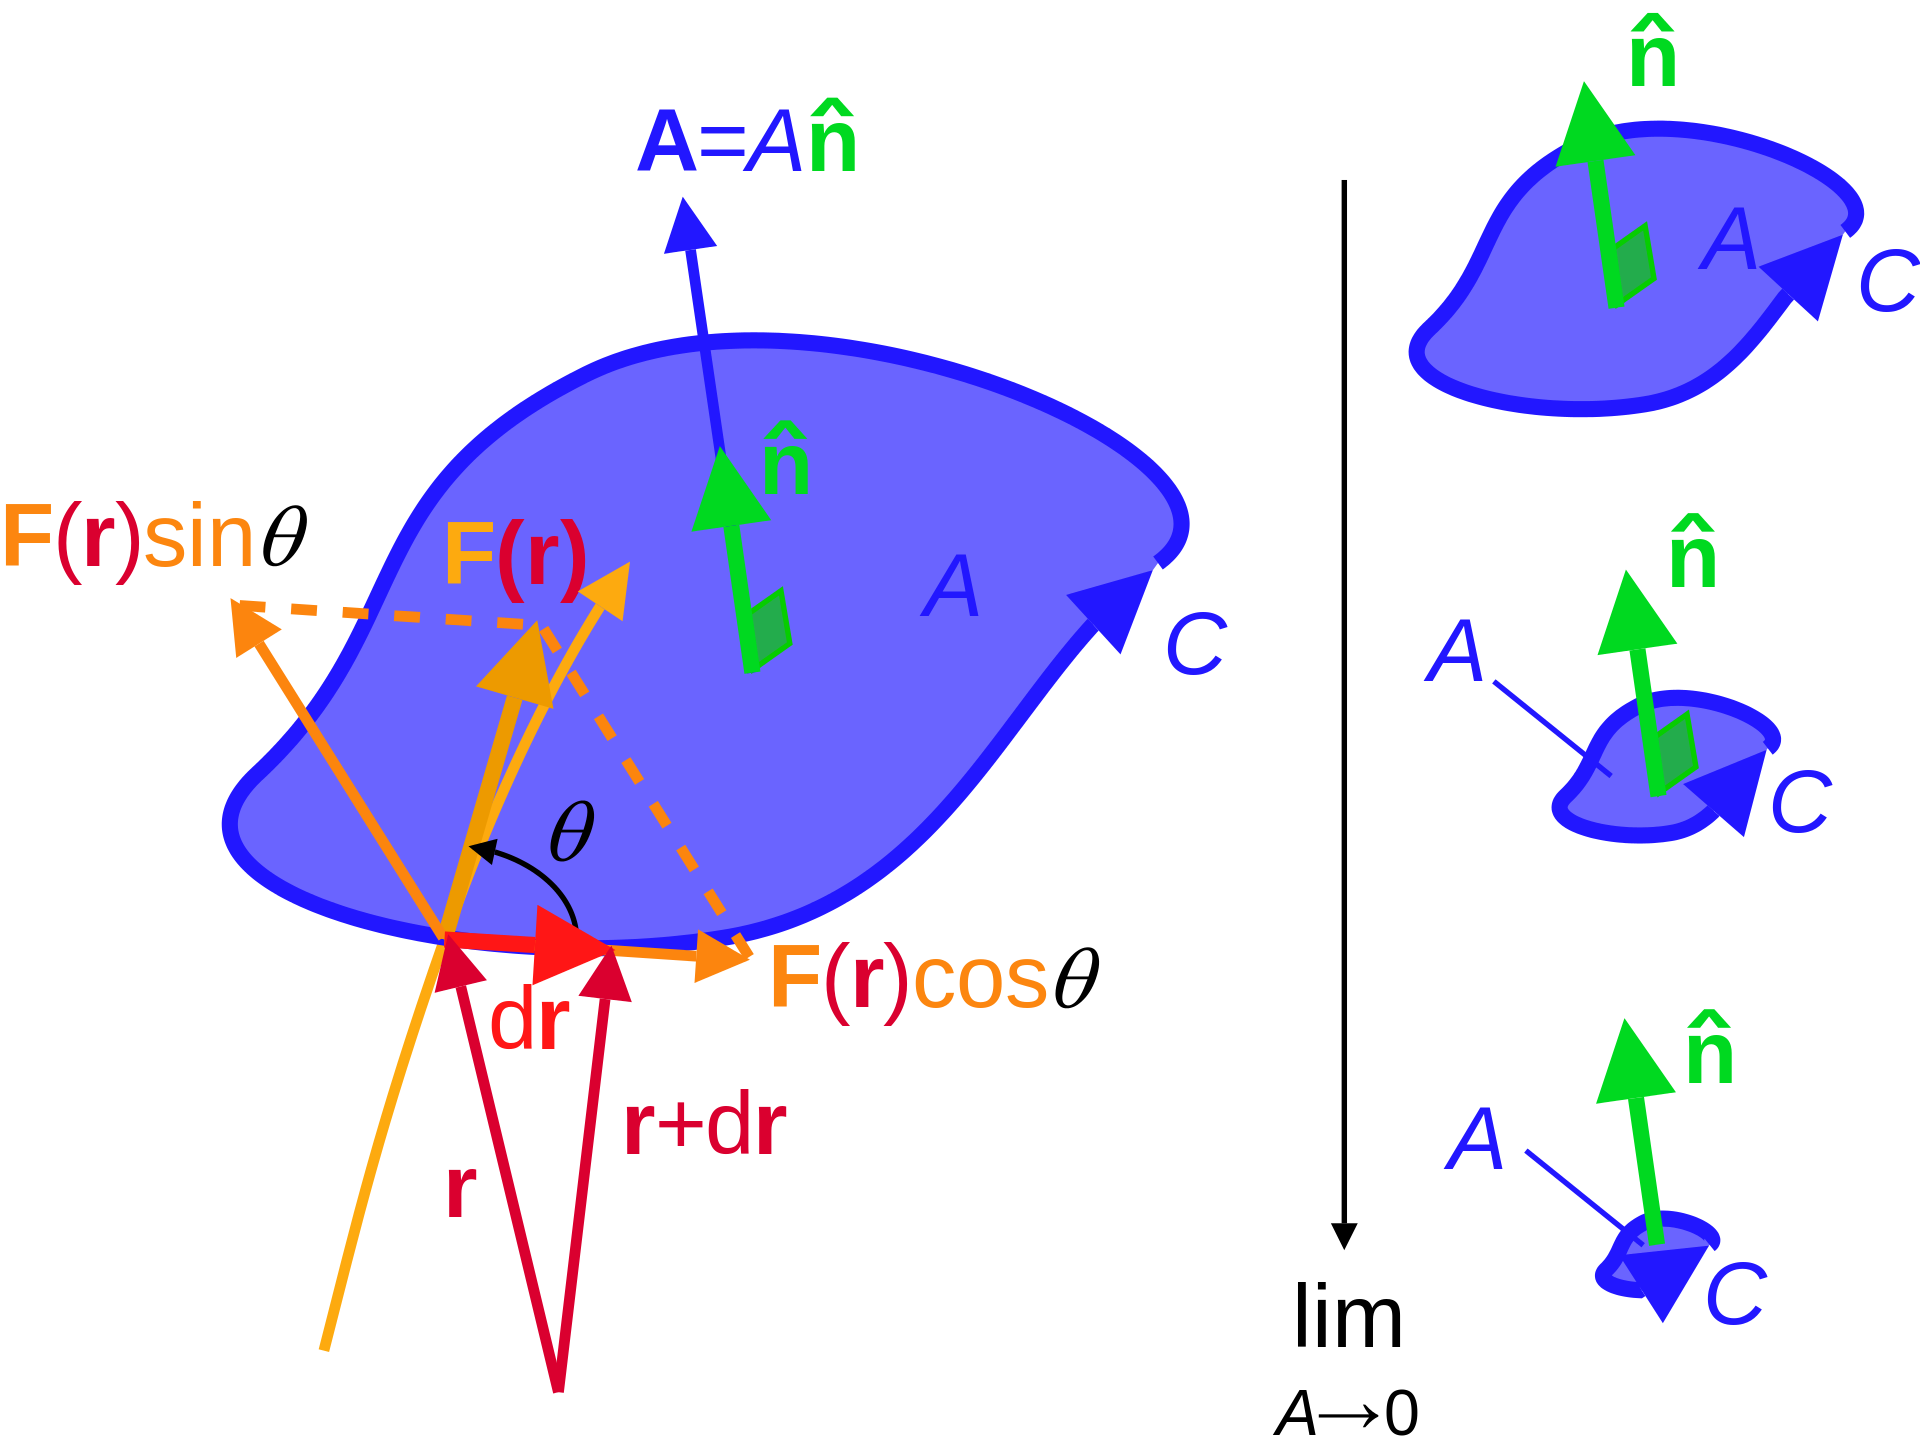
\includegraphics[width=0.4\linewidth]{figures/curl-limit.png}}
    \qquad
    \raisebox{-0.5\height}{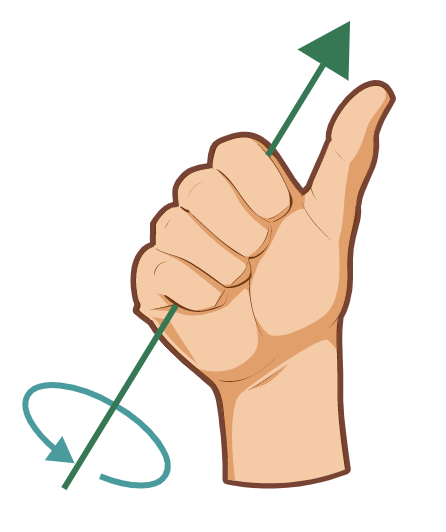
\includegraphics[width=0.2\linewidth]{figures/curl-righthand.png}}
    \caption{From left to right: simple diagram showing relationship between curl and vector field; curl as a limit; the right-hand rule for determining particle rotation.}
    \label{fig:curl}
\end{figure}

\subsection{Properties}
There are some properties involving grad, div, and curl

\begin{theorem}[Sum rules]
$$
\begin{aligned}
\Grad(f+g) &= \Grad(f) + \Grad(g) \\
\Div(\vv F + \vv G) &= \Div(\vv F) + \Div(\vv G) \\
\Curl(\vv F + \vv G) &= \Curl(\vv F) + \Curl(\vv G) \\
\end{aligned}
$$
\end{theorem}

\begin{theorem}[Product rules]
$$
\begin{aligned}
\Grad (fg) &= f \Grad g + g \Grad f  \\
\Div (f\vv G) &= f\Div \vv G + (\Grad f) \cdot \vv G   \\
\Curl (f\vv G) &= f \Curl \vv G +(\Grad f) \times \vv G \\
\Div(\vv F\times \vv G)&= \vv G\cdot \Curl \vv F - \vv F\cdot \Curl \vv G\\
\Curl(\vv F\times \vv G)&=
(\vv G\cdot \nabla)\vv F + (\Div \vv G)\vv F+
(\vv F\cdot \nabla)\vv G + (\Div  \vv F) \vv G \\
\Grad(\vv F\cdot \vv G) &=
(\vv G\cdot \nabla)\vv F + \vv G\times \Curl \vv F -
(\vv F\cdot \nabla)\vv G - \vv F\times \Curl \vv G 
\end{aligned}
$$
where
$$
(\vv F\cdot \nabla)\vv G = \sum_{j=1}^3 F_j \partial_j \vv G,
\qquad 
(\vv G\cdot \nabla)\vv F = \sum_{j=1}^3 G_j \partial_j \vv F.
$$
\end{theorem}

\begin{definition}[Laplacian]
For a twice-differentiable function $f:\; \R^n \to \R$, the Laplacian of $f$ is
$$
\Div(\Grad(f)) = \nabla \cdot (\nabla f) = \nabla^2 f = \Delta f = \sum_{j=1}^n \partial_{jj}f
$$
For $f:\; \R^3 \to \R$,
$$
\Delta f = \nabla^2 f = \frac{\partial^2 f}{\partial x^2} + \frac{\partial^2 f}{\partial y^2} + \frac{\partial^2 f}{\partial z^2}
$$
$\Div(\Grad()),\, \nabla \cdot \nabla,\, \nabla^2,\, \Delta$ are all acceptable notations for Laplacian. $\nabla^2$ is often used in mathematics, and $\Delta$ is more often used in physics.
\end{definition}

In addition, we have the following properties:

The curl of a gradient is zero.
$$
\nabla \times (\nabla \vv F) = \Curl(\Grad(\vv F)) = 0
$$

The divergence of a curl is also zero.
$$
\nabla \cdot (\nabla \times \vv F) = \Div(\Curl(\vv F)) = 0
$$

\section{Conservative Vector Fields}

The divergence and curl of a vector field can be used to understand some of the properties of vector fields. An important family of vector fields are called conservative vector fields.

\begin{definition}[Conservative vector fields]
A vector field $\vv F$ is called conservative if it is the gradient of some scalar function. That is, if there is a function $f$ such that
$$
\nabla f = \vv F = \left( \partialderiv{f}{x},\, \partialderiv{f}{y},\, \partialderiv{f}{z} \right)
$$
The function $f$ is called the potential function of $\vv F$.
\end{definition}

The are some theorems that allow us to show that a vector field is conservative.

\begin{theorem}
Let $\vv F = P\vv i + Q\vv j = (P,Q)$ be a vector field. If $\vv F$ is conservative and $P(x,y)$, $Q(x,y)$ have continuous first-order partial derivatives on a domain $D$, then throughout $D$ we have
$$
\partialderiv{P}{y} = \partialderiv{Q}{x}
$$
The converse of this theorem is not necessarily true. But given some additional constraints, it becomes true.
\end{theorem}

\begin{theorem}
Let $\vv F = P\vv i + Q\vv j = (P,Q)$ be a vector field. Let $D$ be an open simply connected region of the plane. If $P(x,y)$, $Q(x,y)$ have continuous first-order partial derivatives on $D$, and throughout $D$ we have
$$
\partialderiv{P}{y} = \partialderiv{Q}{x}
$$
Then, $\vv F$ is a conservative vector field.
\end{theorem}

\section{Line Integral}

\subsection{Line Integral of Scalar Field}

A line integral of a scalar field or of a function $f(x,y)$ is represented as
$$
\int_C f(x,y) ds
$$


\begin{definition}[Line integral]

If $f$ is defined on a smooth curve $C$ given by a parametric equation
$$
x = x(t) \qquad y = y(t) \qquad a \leq t \leq b
$$
for some $a,b \in \R$, or equivalently by the vector equation $\vv r(t)=(x(t),y(t))$, then the line integral of $f$ along $C$ is
$$
\int_C f(x,y) ds = \lim_{n\to\infty} \sum_{i=1}^n f(x_i^*, y_i^*) \Delta s_i
$$
if this limit exists.
\end{definition}

Using the arc length formula, we know that the length of $C$ is
$$
\int_a^b \sqrt{\left( \frac{dx}{dt} \right)^2 + \left( \frac{dy}{dt} \right)^2} dt
$$
Then we can rewrite the definition as
$$
\int_C f(x,y) ds = \int_a^b \left[ f(x(t),y(t)) \sqrt{\left( \frac{dx}{dt} \right)^2 + \left( \frac{dy}{dt} \right)^2} \right] dt
$$

\subsection{Line Integral of Vector Field}

\begin{definition}[Line integral of vector field]
Given a vector field $\vv F:\; S \to \R^n$, and a curve $C \subset S \subseteq \R^n$ parameterized by $\vv g$, we define the line integral of $\vv F$ over $C$ as
$$
\int_C \vv F \cdot dx = \int_a^b  \vv F(\vv g(t)) \cdot \vv{g}'(t) dt
$$
\end{definition}

\section{The Fundamental Theorem of Line Integral}

\begin{theorem}[The Fundamental Theorem of Line Integral]
Suppose that $f:\; \R^n  \to \R$ is a function of class $C^1$, and that $C$ is a curve oriented by $\vv x = \vv g(t)$ where $a \leq t \leq b$. Then, we can compute the line integral of the vector field $\vv F = \nabla f$ as follows
$$
\begin{aligned}
\int_C \nabla f \cdot d\vv x &= \int_a^b  \nabla f(\vv g(t)) \cdot \vv g'(t)dt \\
&= \int_a^b \frac{d}{dt} f(\vv g(t)) dt & \text{by Chain Rule} \\
&= f(\vv g(b)) - f(\vv g(a)) & \text{by FTC}
\end{aligned}
$$
\end{theorem}

This theorem tells us two things:
\begin{itemize}
    \item The line integral over a conservative vector field does not depend on the path. It only depends on the starting and end points. More formally, if $C_1= \vv r_1(t)\; a \leq t \leq b$ and $C_2 = \vv r_2(t) \; c \leq t \leq d$ are two continuous curves such that $r_1(a)=r_2(c)$ and $r_1(b)=r_2(d)$, that is the curves have the same initial and end points, then if $\vv F$ is a conservative vector field,
    $$
    \int_{C_1} \vv F \cdot d\vv r = \int_{C_2} \vv F \cdot d\vv r
    $$
    This property is called independence of paths.
    \item If $C$ is a continuous path with initial point $\vv r(a)$ and end point $\vv r(b)$, and we denote by $-C$ the curve starts at $\vv r(b)$ and ends at $\vv r(a)$, then for every conservative vector field $\vv F$
    $$
    \int_{-C} \vv F \cdot d\vv r = -\int_C \vv F \cdot d\vv r
    $$
    In other words, changing the orientation of $C$ only changes the sign of the line integral.
    \item For any closed curve $C$, if the vector field $\vv F$ is conservative, then
    $$
    \oint_C \vv F \cdot d\vv r = 0
    $$
\end{itemize}

\section{Green's Theorem}

\begin{definition}[Stokes' orientation]
Given a regular region with piecewise smooth boundary, we define the Stokes' orientation to be the orientation of the boundary such that the interior of the set is always on the left of the direction of travel.
\end{definition}

\begin{theorem}[Green's Theorem]
Let $C$ be a Stokes oriented, piecewise-smooth, simple closed curve in the plane and let $D$ be the region bounded by $C$. If $P(x,y)$ and $Q(x,y)$ have continuous derivatives on an open region that contains $D$ and define $\vv F=(P,Q)$, then
$$
\oint_C \vv F \cdot d\vv r = \oint_C P \, dx + Q \, dy = \iint_D \left( \partialderiv{Q}{x} - \partialderiv{P}{y} \right) dA
$$
\end{theorem}

\section{Stokes' Theorem}

\begin{theorem}[Stokes' Theorem]
Let $S$ be a Stokes oriented piecewise-smooth surface that is bounded by a simple, closed, piecewise-smooth boundary curve $\partial S$. Let $\vv F$ be a vector field whose components are $C^1$ on an open region in $\R^3$ that contains $S$. Then,
$$
\int_{\partial S} \vv F \cdot d\vv r = \iint_S \Curl \vv F \cdot d\vv S = \iint_S \Curl \vv F \cdot \hat{n}\, dA
$$
\end{theorem}

